\begin{figure}[h!]
    \centering
    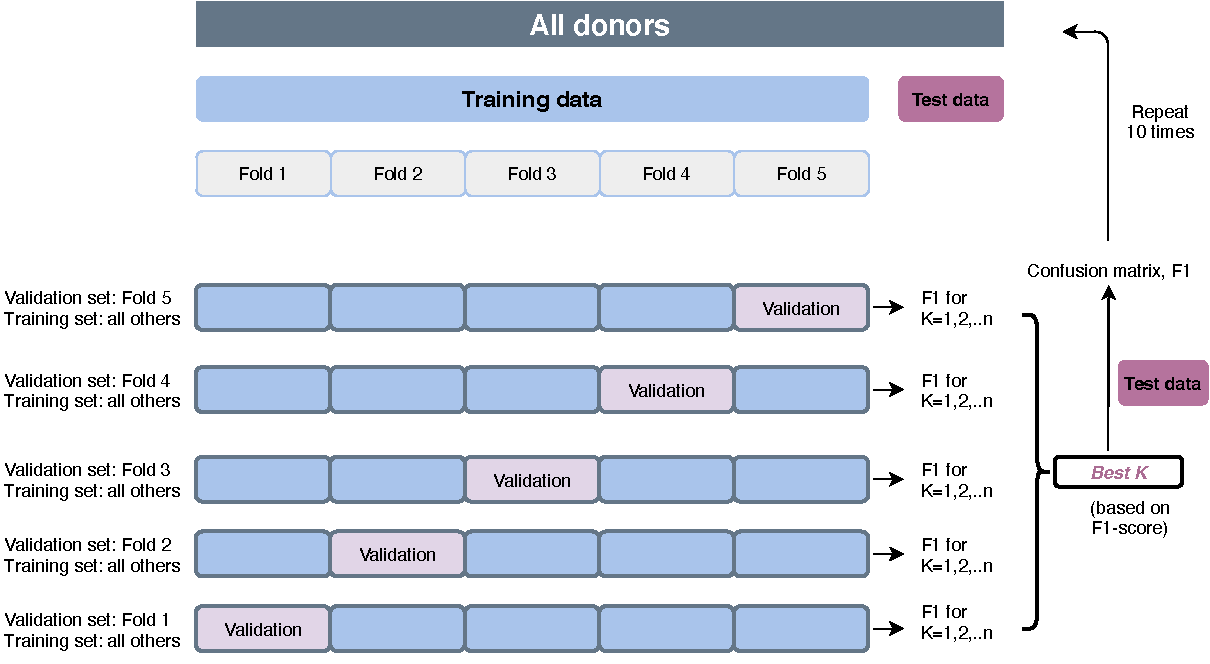
\includegraphics[scale=0.78]{graphics/ML_demo.pdf}
    \caption{\textbf{Illustration of machine learning cross validation workflow.} Data was split into a test set (1/10) and a training set (9/10). The training set was divided into 5 folds, each fold was sequentially used as a validation set to select the parameter $K$ of the model. From the set of $F1$'s for each $K$, I selected the best $K$. This $K$ was then applied to the test set for final evaluation (1/10 of the data). The whole process was repeated 10 times to evaluate the possible range of the accuracy, reported in the form of confusion matrices or $F1$.}
    \label{fig:cv_demo}
\end{figure}
